This section describes the theoretical formalism which predicts the transverse emittance growth in the presence of $\CC$ RF noise. First, it introduces the concept of noise in accelerator beam dynamics. The second section focuses on the $\CC$ noise both in amplitude and phase and it provides the equations with which one can estimate the noise-induced emittance growth. The last section, comments briefly on the experiments that took place in KEKB as it's the only time this issue was treated in the past. 



%You need the frist section to introduce the dipole noise as you will apply it in the simulations.
\section{Noise}\label{sec:noise_definition}
%External noise means that it is independent of the beam itself.
In particle accelerators, a major issue of concern is the presence of external noise as it leads to transverse emittance growth, particle losses and limits the beam lifetime. Examples of noise sources are ripples in the power converter ripples which lead to fluctuations of the magnetic fields, ground motion, and various instruments in the accelerator structure such as the transverse damper and the Crab Cavities. % sofias's thesies introduction of chatper 5.
%Ripples in the power supply voltage are converted into current ripples, depending on the magnet's impedance, which eventually leads to magnetic field perturbations through the magnet's transfer function (vacuum chamber, beam screen). sofia's thesis p.95

From the various noise sources that are present in an accelerator, this thesis focuses on the dipolar noise and mainly on the CC noise. Dipolar noise is the one produced by the majority of the noise sources and is constant along the bunch, i.e. all the particles are affected the same way. % this noise is also referred to as rigid noise 
On the other hand, the way the CC noise affects the particles depends on their longitudinal position within the bunch (more details in the following paragraphs).

%Therefore, in the following the term "noise" refers to a sequence of random kicks (stochastic process) that affect the particles within a bunch by changing their transverse momentum each turn as follows.
Past studies~\cite{Lebedev:248620, Lebedev:248622, PhysRevSTAB.18.101001} have dealt with this type of noise in the context of the induced emittance growth theoretically and in simulations. It has been shown, that the noise can be modeled as a sequence of random kicks (stochastic process) that affect the particles within a bunch by changing their transverse momentum each turn as follows:
\begin{equation}\label{eq:external_noise_kicks}
    u^\prime_1 =  u^\prime_0 + \Delta u^\prime,
\end{equation}
where $u=(x,y)$ denoting the horizontal and vertical plane and $\Delta u^\prime$ is the change of the momentum due to the noise in units of rad. In this thesis the term "noise" refers to the above mentioned stochastic process.
% This approach will be used in the following. In th
% if it is dipole noise it is oftern written: Delta u = thera


\section{Crab Cavity noise and emittance growth}\label{eq:CC_noise_intro}
As already mentioned in the Introduction (Section~\ref{sec:motivation_outline}) the presence of noise in the $\CC$ low-level RF system is an issue of major concern for the HL-LHC project as it results in transverse emittance growth and subsequently in loss of luminosity. To this end, in 2015, P.~Baudrenghien and T.~Mastoridis developed a theoretical model~\cite{PhysRevSTAB.18.101001} which predicts this transverse emittance growth induced by $\CC$ noise focusing on the HL-LHC scenario. In particular, the model assumes a hadron machine, zero synchrotron radiation damping, long bunches (in the order of cm), and white RF noise (discrete spectral lines are excluded).  Additionally, it is assumed that the $\CC$ RF zero phase is set at the center of the bunch.

\textbf{White noise}\\
In signal analysis, white noise is a random signal with the same amplitude (intensity) at all the frequencies which results in a constant power spectral density. For the computational analysis (i.e. simulation studies), the signals are sampled at a finite number of points which are called discrete-time signals. In discrete-time, the white noise can be considered as a sequence of uncorrelated random variables taken from a Gaussian distribution with zero mean and finite standard deviation. More details on the continuous and discrete time analysis and the term of the power spectral density can be found in Appendix~\ref{ch:app_B}. The definition for the standard deviation of a distribution can be found in Appendix~\ref{ch:app_A}.

It should be highlighted, that the above mentioned model is also applicable to the SPS (where the same conditions apply), where the $\CC$s will be tested before their installation in the LHC (Section~\ref{sec:motivation_outline}). % Thus, the results from the SPS $\CC$ tests can be used for scaling to the HL-LHC case.
The equations and formulas from the theoretical model that are essential for the understanding of the studies are discussed below.


\subsection{Crab Cavity amplitude and phase noise}\label{subsec:AN_PN}
The unperturbed instantaneous $\CC$ voltage equals the one of an ideal oscillator:
\begin{equation}\label{eq:CC_voltage_t}
    V_\mathrm{CC}(t) = \CCvoltage \sin{\left ( 2 \pi \CCfrequency t \right )},
\end{equation}

where $\CCvoltage$ is the peak amplitude of the $\CC$ voltage and $\CCfrequency$ the $\CC$ frequency. Equation~\eqref{eq:CC_voltage_t} can be re-written as a function of the longitudinal position within the bunch $z$ instead of time $z$ as follows:
\begin{equation}\label{eq:CC_voltage_z}
    V_\mathrm{CC}(z) = \CCvoltage \sin{\left ( \frac{2\pi \CCfrequency}{\beta_0 c}z \right )},
\end{equation}
where $\beta_0$ is the relativistic parameter and $c$ is the speed of light. The above equation is obtained as: $z=v \cdot t \Rightarrow t=z/v=z/(\beta_0 c)$.
In the presence of modulations in amplitude and phase Eq.~\eqref{eq:CC_voltage_z} becomes (details in Appendix~\ref{app:Measured_noise}):
\begin{equation}\label{eq:CC_voltage_z}
    V_\mathrm{CC}(z) = \CCvoltage (1+\Delta A) \sin{\left ( \frac{2\pi \CCfrequency}{\beta_0 c}z + \Delta \phi \right )},
\end{equation}

where $\Delta \phi$ is the deviation from the nominal phase, $2\pi \CCfrequency z/(\beta_0 c)$, and will be referred to as phase noise in the following. $\Delta A = \Delta \CCvoltage / \CCvoltage$ is the relative deviation from the nominal amplitude $\CCvoltage$ and will be referred to as amplitude noise. The units od $\Delta \phi$ is $\mathrm{rad^2}$ while $\Delta A$ has no units as it's a relative quantity.
% Note on the above paragraph: source that ΔA = ΔV/V: https://www.osti.gov/servlets/purl/1846026/
% The units of ΔΑ and Δφ are shown in Table II of the paper of Themis and Philippe.


In the calculation of the RF noise effects it is assumed that RF phase and amplitude noises are independent. The validity of this hypothesis depends on the actual architecture of the LLRF responsible for the regulation of the cavity field. This is presently being designed at CERN. Further details can be found in Ref.~[15] of the above-mentioned publication of Baudrenghien and Mastoridis~\cite{PhysRevSTAB.18.101001}, but discussing them is out of the scope of this thesis.
 

%Due to the $\CC$ RF noise sources in the LHC, HL-LHC and, SPS machines, the amplitude and phase noise spectra can be considered  independent, and thus they can be treated separetatly. The technical details can be found in Ref.~[15] of the above-mentioned publication of Baudrenghien and Mastoridis~\cite{PhysRevSTAB.18.101001}, but discussing them is out of the scope of this thesis.
% 1) You need to understand Ref.[15]
% 2) Q and I demodulator --> it enables easily extracting instantaneous amplitude and phase over time. source: https://indico.cern.ch/event/781242/contributions/3251767/attachments/1780299/2896017/Powerpoint_1.pdf
% 3) Document on the digital Q/I demodulator, that might be useful when you try to understand it. https://accelconf.web.cern.ch/p95/ARTICLES/RPQ/RPQ02.PDF

To this end, and following the analysis in Ref.~\cite{PhysRevSTAB.18.101001} and in accordance with Eq.~\eqref{eq:external_noise_kicks} the phase and amplitude noise kicks on each particle within a bunch can be modeled as the following kicks on the momentum: % at the location of the CC; s=s_CC. Eq.7 in ref~\cite{PhysRevSTAB.18.101001} but for not normalised co-oridnates.
% Presetnation: https://docs.google.com/presentation/d/1Jv0Es99utlZSSg25_9oplI53A5MdPDfJSjsSneRXaV8/edit#slide=id.gbb99f3cf0a_0_65
\begin{equation}\label{eq:amplitude_noise_kick}
  \textbf{\textrm{Amplitude noise:}} \  u^\prime_1 =  u^\prime_0 + A \sin{\left (  \frac{2 \pi \CCfrequency}{c \beta_0}z   \right )},
\end{equation}
\begin{equation}\label{eq:phase_noise_kick}
    \textbf{\textrm{Phase noise:}} \ u^\prime_1 =  u^\prime_0 + A \cos{\left (  \frac{2 \pi \CCfrequency}{c \beta_0}z   \right )},
\end{equation}

where $u^\prime$, with $u=(x,y)$, is the normalised transverse momentum and $z$ the longitudinal co-ordinate of each particle as defined in Eq.~\eqref{eq:particle_coordinates}, $\CCfrequency$ is the $\CC$ frequency, $c$ is the speed of light and $\beta_0$ the relativistic $\beta$. Finally, $A=\CCvoltage /(E_b \cdot \Delta A )$ or $A=\CCvoltage /(E_b \cdot \Delta \phi )$ the scaling factor for amplitude or phase noise respectively. The typicall value of $A$ that will be used in the simulations later is $10^{-8}$.

% The following paragraph is inspired by what I said in the IPAC talk.
Figure~\ref{fig:amplitude_noise} and Fig.~\ref{fig:phase_noise} provide a schematic visualisation of the amplitude and phase noise respectively along with the impact of their kicks on the particles. It can be seen that in the presence of amplitude noise the head and the tail of the bunch are kicked in opposite directions which results in intra-bunch oscillations. On the other hand, in the presence of phase noise, the particles in the bunch receive kicks that are in phase. This results in a shift of the bunch centroid which basically is a dipole or mode 0 motion.

\begin{figure}[!h] % at the directory of ipac22
    \centering         
    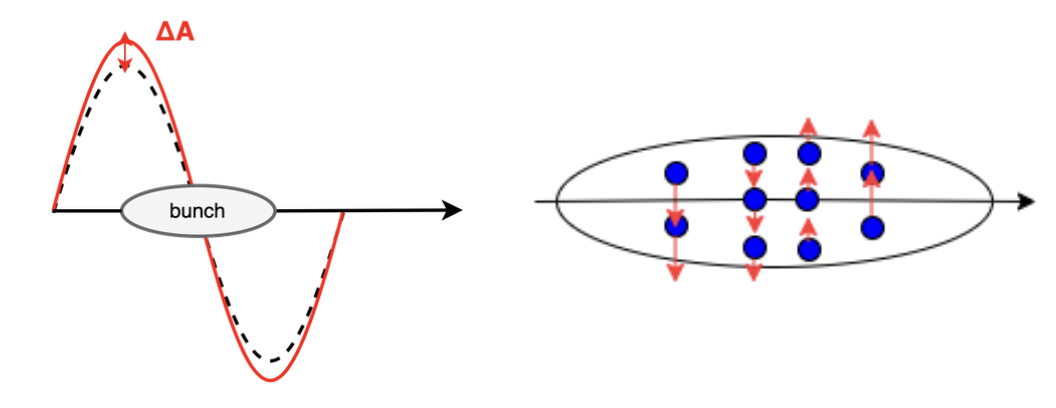
\includegraphics[width=0.8\textwidth]{images/Ch3/amplitude_noise.png}
        \caption{Modulation in amplitude or amplitude noise (left) and its impact on the particles within the bunch (right). The blue dots represent the individual particles while the red arrows indicate the direction of the noise kicks which act on them.}
        \label{fig:amplitude_noise}
 \end{figure}

 \begin{figure}[!h] % at the directory of ipac22
    \centering         
    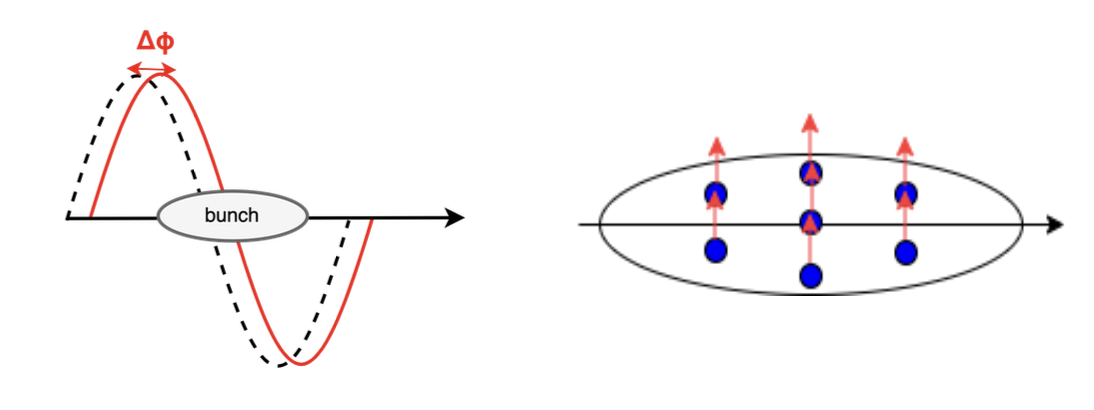
\includegraphics[width=0.85\textwidth]{images/Ch3/phase_noise.png}
        \caption{Modulation in phase or phase noise (left) and its impact on the particles within the bunch (right). The blue dots represent the individual particles while the red arrows indicate the direction of the noise kicks which act on them.}
        \label{fig:phase_noise}
 \end{figure}

 Finally, it is worth mentioning, that for the LHC, HL-LHC and SPS $\CC$s the amplitude and phase RF noise are represented by white noise spectra. In that case, they can be considered as a sequence of uncorrelated random variables taken from a Gaussian distribution with zero mean and standard deviation $\sigma_{\Delta A}$ and  $\sigma_{\Delta \phi}$ respectively which equals the total noise power (see Appendix~\ref{app:discrete_time_analysis} for definitions). % sampled by the beam, as also written here: https://www.osti.gov/servlets/purl/1846026 

\subsection{Emittance growth formulas}\label{subsec:CC_emit_growth_theoretical_formulas}
As already mentioned, the theoretical formalism for predicting the transverse emittance growth in the presence of $\CC$ RF amplitude and phase noise was derived in Ref.~\cite{PhysRevSTAB.18.101001}. The derivation assumes a single bunch, that the noise kicks are represented by a stochastic process, zero coupling between the horizontal and vertical plane, the beam energy is constant (no acceleration) and, $\CC$ RF zero phase is at the center of the bunch, $z=0$ and a uniform noise spectrum across the betatron tune distribution. 
% One more assumption that I didn't write Inthe analysis presented in this work, the density function is independent of time (paper of themis and philippe p.2) i didn't write it in the assumption.

Taking these conditions into account, the emittance growth resulting from amplitude noise is estimated from:
\begin{equation}\label{eq:dey_an}
    \frac{d\epsilon^{\mathrm{geom}}_u}{dt}  = \beta_{u, \mathrm{CC}} \left( \frac{e\CCvoltage\frev}{2E_b}\right)^2 \!\! C_{\Delta A} (\sigma_{\phi}) \!\! \sum_{k=-\infty}^{+\infty} S_{\Delta A}[(k \pm \widebar{Q}_u \pm \widebar{Q}_s)\frev].
\end{equation}
For phase noise, the emittance growth is estimated from:
\begin{equation}\label{eq:dey_pn}
    \frac{d\epsilon^{\mathrm{geom}}_u}{dt}  = \beta_{u, \mathrm{CC}}  \left( \frac{e\CCvoltage\frev}{2E_b}\right)^2 C_{\Delta \phi} (\sigma_{\phi}) \sum_{k=-\infty}^{+\infty} S_{\Delta \phi}[(k \pm \widebar{Q}_u) \frev].
\end{equation}
In these formulas, which are valid for both transverse planes as $u=(x,y)$, $\beta_{u, \mathrm{CC}}$ is the transverse beta function at the location of the CC, $\CCvoltage$ the CC voltage, $\frev$ the revolution frequency of the beam, $E_b$ the beam energy, and $\widebar{Q}_u$ and $\widebar{Q}_s$ the mean of the betatron and synchrotron tune distribution \footnote{For white noise spectra the effect of noise is independent of the actual tune distribution, hence the use of the mean quantities. The generic formulas can be found in Ref.~\cite{PhysRevSTAB.18.101001}}. %p.6-7 In the paper of Themis and Philippe.
The $\pm$ signs refer to the upper $(+)$ and lower $(-)$ sidebands of the betatron and synchrobetatron frequencies. $S_{\Delta A}$ and $S_{\Delta \phi}$ are the power spectral densities (PSD) of the noise at all the betatron and synchrobetatron (for the amplitude noise case) sidebands and they are expressed in units of Hz$^{-1}$ and rad$^2$Hz$^{-1}$, respectively. The definition of the power spectral density along with the fundamental terminology for the signal-processing can be found in Appendix~\ref{ch:app_B}\footnote{In the Appendix amplitude and phase noise are noted with just $\alpha$ and $\phi$, instead of $\Delta A$ and $\Delta \phi$, for simplicity.}.
$C_{\Delta A}$ and $C_{\Delta \phi}$ are correction terms to account for the bunch length:
\begin{align}
C_{\Delta A}(\sigma_{\phi}) = ~& e^{-\sigma_{\phi}^2}\sum_{l=0}^{+\infty} I_{2l+1}(\sigma_{\phi}^2),\\
C_{\Delta \phi}(\sigma_{\phi}) = ~& e^{-\sigma_{\phi}^2} \left[I_0(\sigma_{\phi}^2) + 2 \sum_{l=1}^{+\infty} I_{2l}(\sigma_{\phi}^2) \right],
\end{align}
with $\sigma_{\phi}$ the rms bunch length, in rad, with respect to the CC frequency $\CCfrequency$, and $I_n(x)$ the modified Bessel function of the first kind. 

Figure~\ref{fig:correction_term_bunch_length} illustrates the correction term for different values of bunch length for amplitude (left) and phase (right) noise. The SPS nominal bunch length used in the CC tests is shown in the orange for reference.

% Figures created using the following script: natriant/cernbox/Project_thesis/plot_bunch_length_correction_term
\begin{figure}[!ht]
    \centering
    \begin{subfigure}[t]{0.45\textwidth}
        \centering
        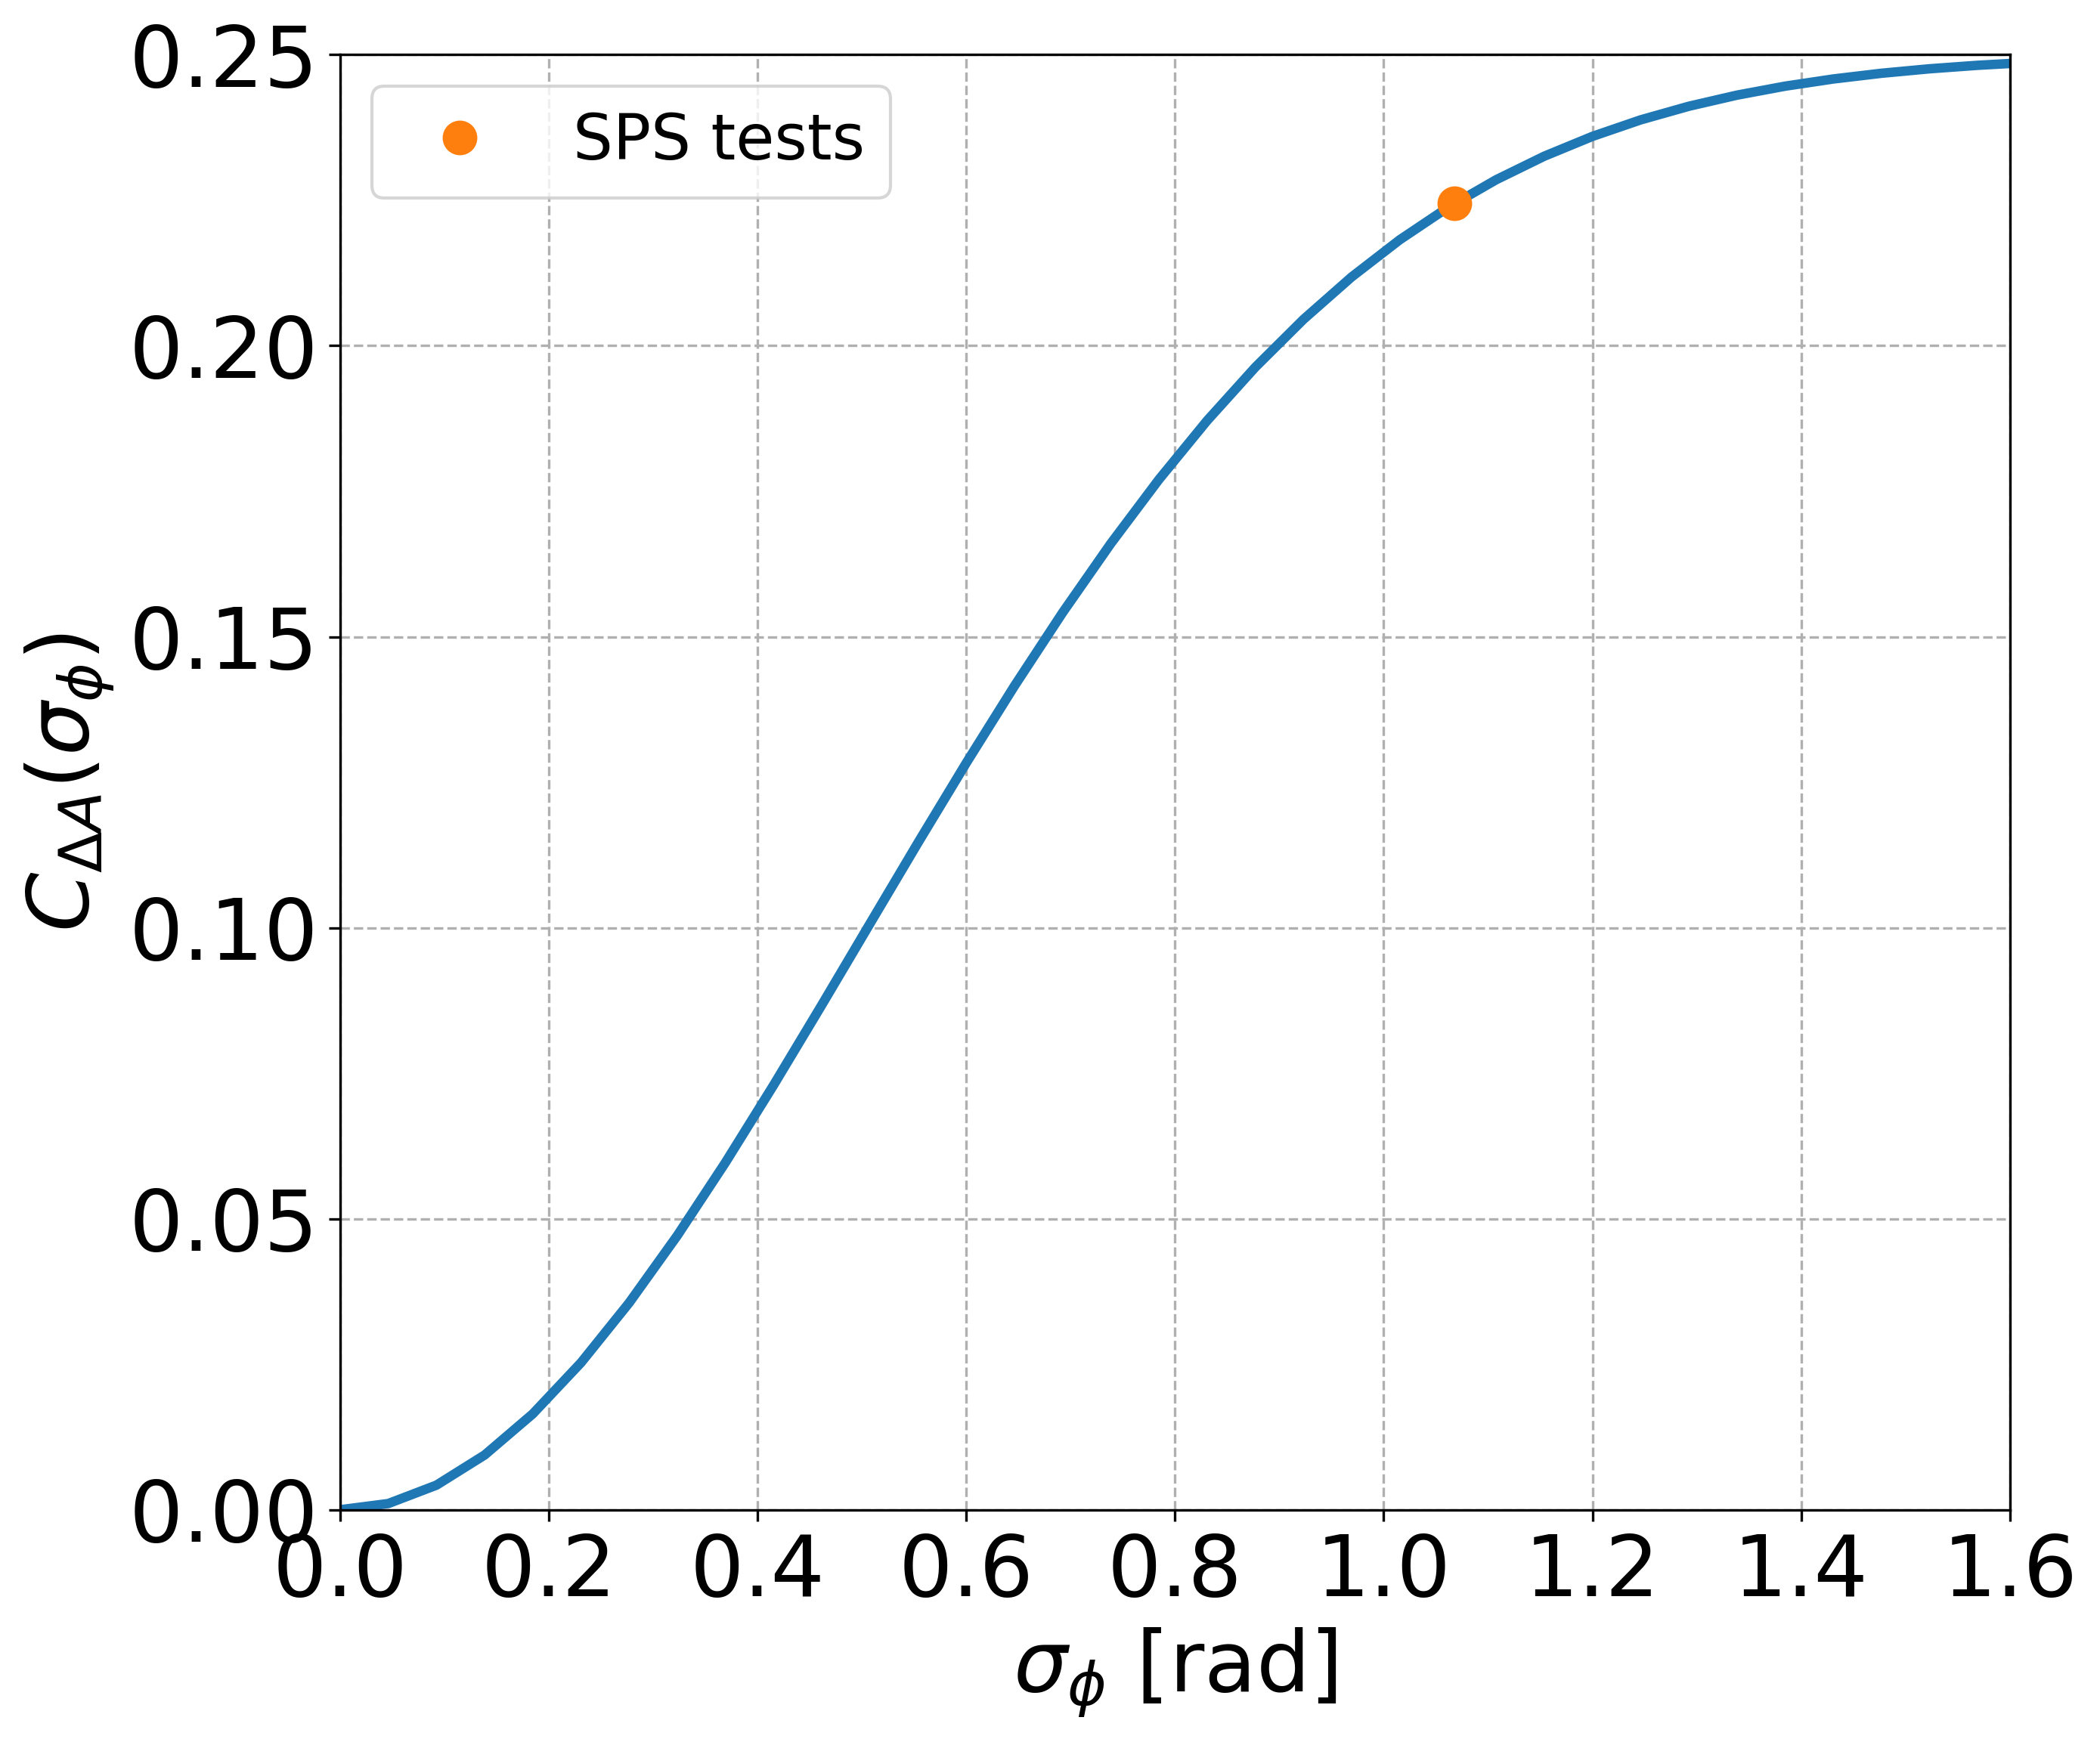
\includegraphics[width=1\textwidth]{images/Ch3/CA_bunch_length_dependence.png}
        %\caption{$y=\sin(2 \pi f t),\ f=50$ Hz}
        %\label{fig:add_label_here}
    \end{subfigure}
    \hfill
    \begin{subfigure}[t]{0.45\textwidth}
        \centering
        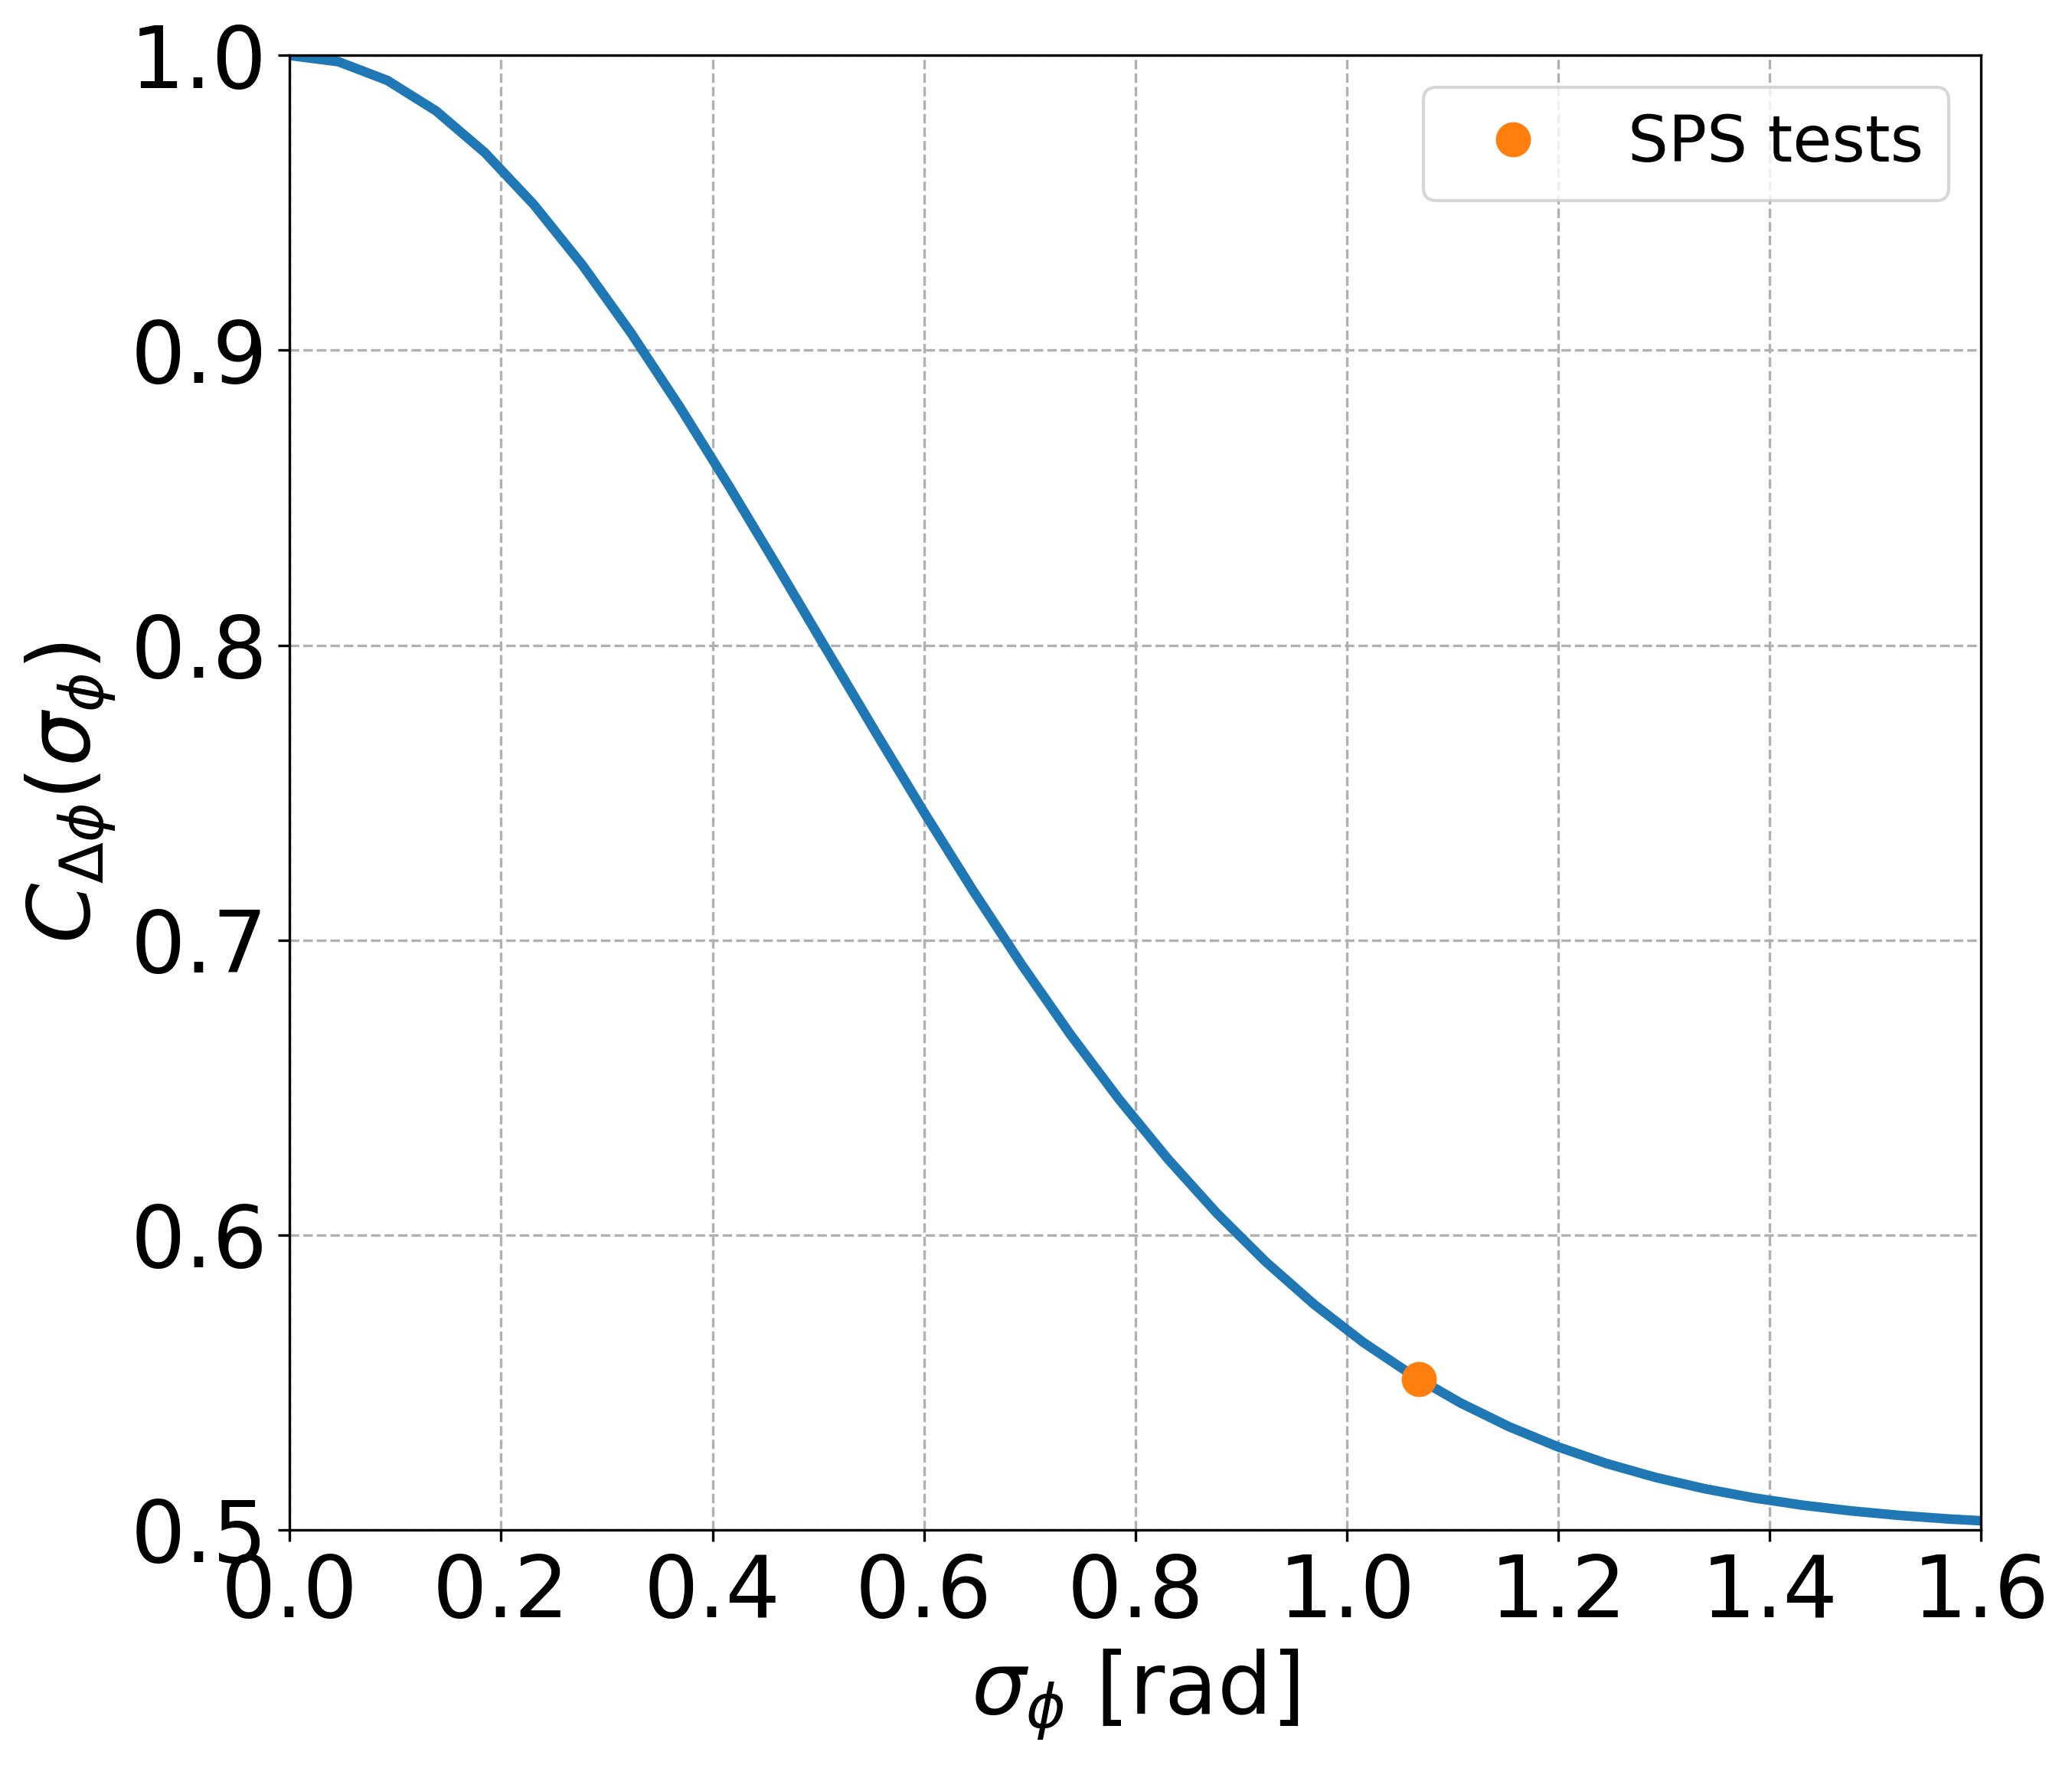
\includegraphics[width=1\textwidth]{images/Ch3/Cphi_bunch_length_dependence.png}
        %\caption{Discrete Fourier transform}
        %\label{fig:add_label_here}
    \end{subfigure}
    \hfill
     \caption{Correction term for amplitude (left) and phase (right) noise over a range of bunch length values.} % bunch passage
     \label{fig:correction_term_bunch_length}
 \end{figure}


\section{Studies in KEKB}\label{eq:past_studies_KEKB}
The $\CC$s have been tested in the past with lepton beams in KEKB in Japan (further references on their operation were given in the Introduction). %~\cite{CC_KEKB_4440798, Funakoshi:1955812, oide:pac07-mozaki01}.
As expected, the sensitivity of the beam to the $\CC$ RF noise was also studied. However, there were significant differences in the conditions in the HL-LHC, LHC, and SPS. In particular, the studies in KEKB were conducted for lepton bunches (instead of hadron bunches), they were about an order of magnitude shorter than the ones of the hadron machines (no effect from amplitude noise), and there was significant damping from the synchrotron radiation and the RF noise was characterised by a single spectral line (instead of white noise). Due to these differences, the studies at KEKB are not applicable to the studies presented in this thesis. Nevertheless, these studies can be found in Ref.~\cite{PhysRevSTAB.14.111003} and they consist the only other available experience with $\CC$ RF noise but going into further details is out of the scope of this thesis.